\documentclass[a4paper]{article}
\usepackage{graphicx}
\usepackage[latin1]{inputenc}
\usepackage{amsmath}
\usepackage{fancyhdr}
\pagestyle{fancy}
\lhead{\textsc{URIsolve App}}
\rhead{\textsc{Node Voltage Method (Supernode approach)}}
\cfoot{www.isep.ipp.pt}
\lfoot{DEE - ISEP}
\rfoot {\thepage}
\renewcommand{\headrulewidth}{0.4pt}
\renewcommand{\footrulewidth}{0.4pt}

\title{
\raisebox{-.2\height}{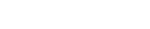
\includegraphics[height=1cm, keepaspectratio]{logo}} URIsolve APP \\
\newline
\textsc{Node Voltage Method} \\
\textsc{(Supernode approach)} \\
Step by Step Solution \\
\vspace*{1\baselineskip}
}

\author{
\begin{tabular}[t]{c@{\extracolsep{8em}}c}
Lino Sousa           & Mário Alves          \\
1140355@isep.ipp.pt  & mjf@isep.ipp.pt      \\
					 &                      \\
André Rocha          & Francisco Pereira    \\
anr@isep.ipp.pt      & fdp@isep.ipp.pt      \\
\end{tabular}
}

\date{}

\begin{document}

\maketitle
\thispagestyle{empty}

\vspace{\fill}
\begin{abstract}
\centering
This document provides a step by step solution for the submitted circuit, using the Node Voltage Method (NVM). If possible, it's implemented the Supernode approach to simplify the circuit analysis.
\end{abstract}
\vspace{\fill}

\begin{center}
\today
\end{center}

\clearpage
\pagenumbering{arabic}

\newpage

\section{Circuit Image}


\section{Circuit Information}

\begin{table}[h!]
\centering
\begin{tabular}{clclclc}
\textbf{Frequency {[}F{]}} &  & \textbf{Current Sources {[}I{]}} &  & \textbf{Ammeters {[}A{]}} &  & \textbf{Simulation {[}AC/DC{]}} \\
F=1GHz                     &  & I=1                              &  & 15/15                     &  & AC
\end{tabular}
\end{table}

\section{Fundamental Variables}

\begin{table}[hbt!]
\centering
\begin{tabular}{clclclc}
\textbf{Branches {[}R{]}} &  & \textbf{Nodes {[}N{]}} &  & \textbf{Isolated Voltage Sources {[}T{]}} &  & \textbf{Equations {[}E{]}} \\
R=15                      &  & N=9                    &  & T=6                                       &  & E=N-T-1=2
\end{tabular}
\end{table}

\section{Supernodes}

\subsection{Floating}

\subsubsection{SNf1}


\paragraph{} Formed by Nodes: {A, B, E, J, H, D}
\par

\paragraph{} Equations:

\begin{gather*}
\begin{cases}
V_{B} = \mathrm{V_{A}}-5\\V_{E} = \mathrm{V_{A}}-4\\V_{J} = \mathrm{V_{A}}-13\\V_{H} = \mathrm{V_{A}}-13\cdot\left( i+1\right)\\V_{D} = \mathrm{V_{A}}-4\\
\end{cases}
\end{gather*}
\par

\paragraph{} Steps:

\begin{gather*}
\begin{cases}V_{B} = \mathrm{V_{A}}- V2\\[0.7em] V_{D} = \mathrm{V_{A}}- V3\\[0.7em] V_{E} = \mathrm{V_{A}}- V2+ V12\\[0.7em] V_{J} = \mathrm{V_{A}}- V6- V2+ V12\\[0.7em] V_{H} = - V2- V10- V6+\mathrm{V_{A}}+ V12\end{cases}
\end{gather*}

\subsubsection{SNf2}

\paragraph{} Formed by Nodes: {T, M}
\par

\paragraph{} Equations:

\begin{gather*}
\begin{cases}
V_{M} = \mathrm{V_{T}}-1
\end{cases}
\end{gather*}
\par

\paragraph{} Steps:

\begin{gather*}
\begin{cases}V_{M} = \mathrm{V_{T}}- V11\end{cases}
\end{gather*}
\par

\subsection{Grounded}
Not found in this circuit.

\newpage
\section{Circuit Currents}

\subsection{General information}

\begin{table}[ht]
\caption{List of the circuit currents and its properties/components}
\centering
\begin{tabular}{cccc}
\textbf{Reference} & \textbf{Start Node} & \textbf{End Node} & \textbf{Components} \\ \hline
I01                & A                   & GND               & V1, L1, V7          \\
I02                & GND                 & B                 & R6                  \\
I03                & GND                 & H                 & C1, I3, R7          \\
I04                & A                   & B                 & V2                  \\
I05                & B                   & H                 & R4                  \\
I06                & H                   & J                 & V10                 \\
I07                & B                   & E                 & V12                 \\
I08                & A                   & D                 & V3                  \\
I09                & D                   & T                 & R1                  \\
I10                & E                   & T                 & R10, C2             \\
I11                & T                   & M                 & R2                  \\
I12                & J                   & M                 & R3                  \\
I13                & D                   & E                 & R9                  \\
I14                & E                   & J                 & V6                  \\
I15                & T                   & M                 & V11
\end{tabular}
\end{table}

\subsection{Equivalent Impedances and Voltages}
\paragraph{} Branch from A to gnd
\begin{gather*}
\begin{cases}
VeqAgnd =  - V1 - V7 = -11\;V
\end{cases}
\end{gather*}
\par

\paragraph{} Branch from D to T
\begin{gather*}
\begin{cases}
VeqDT =  - V4 - V5 = -8\;V
\end{cases}
\end{gather*}
\par

\paragraph{} Branch from E to T
\begin{gather*}
\begin{cases}
ZeqgndH = R10 + C2  = 50 - 159.155i\;\Omega
\end{cases}
\end{gather*}
\par

\paragraph{} Branch from gnd to H
\begin{gather*}
\begin{cases}
ZeqgndH = C1 + R7  = 5 - 159.155i\;\Omega
\end{cases}
\end{gather*}
\par
newpage
\subsection{Equations}
Equations using the Kirchhoff Nodes Law (KNL)

\subsubsection{Node SNf1}
\begin{figure}[hbt]
\centering{\includegraphics[height=4cm, keepaspectratio]{snf1}}
\caption{Node SNf1 currents}
\label{snf1currents}
\end{figure}
\begin{equation}
  I01+I09+I10+I12=I02+I03
\end{equation}

\subsubsection{Node SNf2}
\begin{figure}[hbt]
\centering{\includegraphics[height=4cm, keepaspectratio]{snf2}}
\caption{Node SNf2 currents}

\label{snf2currents}
\end{figure}
\begin{equation}
  I09+I10+I12=0
\end{equation}

\newpage
\section{Equation System}

\paragraph{} Equations:
\begin{gather*}
\begin{cases}\frac{\left(\mathrm{V_{A}}- V1- V7\right)}{ XL1}+\left(\frac{\mathrm{V_{B}}}{ R6}\right)+\frac{\left( V_{D}- V4- V5-\mathrm{V_{T}}\right)}{ R1}+\frac{\left( V_{E}-\mathrm{V_{T}}\right)}{ XC2}+\frac{\left(\mathrm{V_{J}}- V_{M}\right)}{ R3}-0.001 = 0 \\[0.7em] \frac{\left( V_{D}- V4- V5-\mathrm{V_{T}}\right)}{ R1}+\frac{\left( V_{E}-\mathrm{V_{T}}\right)}{ XC2}+\frac{\left(\mathrm{V_{J}}- V_{M}\right)}{ R3} = 0\end{cases}
\end{gather*}
\par

\paragraph{} Steps:

%\hfill\begin{minipage}{\dimexpr\textwidth-1cm}
\begin{small}\textbf{\textit{Step 1:}}\end{small}  Reorder current equations
\begin{gather*}
\begin{cases}I01 - I02 + I09 + I10 + I12 - I03 = 0 \\[0.7em] I09 + I10 + I12 = 0\end{cases}
\end{gather*}

\begin{small}\textbf{\textit{Step 2:}}\end{small}  Substitute the known currents
\begin{gather*}
\begin{cases}I01 - I02 + I09 + I10 + I12 - 0.001 = 0 \\[0.7em] I09 + I10 + I12 = 0\end{cases}
\end{gather*}

\begin{small}\textbf{\textit{Step 3:}}\end{small}  Compute the remaining currents using Ohm's Law
\begin{gather*}
\begin{cases}I01 = \frac{\left(\mathrm{V_{A}}- V1 -  V7\right)}{ XL1} \\[0.7em] I02 = -\left(\frac{\mathrm{V_{B}}}{ R6}\right) \\[0.7em] I09 = \frac{\left( V_{D}- V4 -  V5 - \mathrm{V_{T}}\right)}{ R1} \\[0.7em] I10 = \frac{\left( V_{E}-\mathrm{V_{T}}\right)}{ XC2} \\[0.7em] I12 = \frac{\left(\mathrm{V_{J}}- V_{M}\right)}{ R3}\end{cases}
\end{gather*}

\begin{small}\textbf{\textit{Step 4:}}\end{small}  Substitute each current by its equation
\begin{gather*}
\begin{cases}\frac{\left(\mathrm{V_{A}}- V1- V7\right)}{ XL1}+\left(\frac{\mathrm{V_{B}}}{ R6}\right)+\frac{\left( V_{D}- V4- V5-\mathrm{V_{T}}\right)}{ R1}+\frac{\left( V_{E}-\mathrm{V_{T}}\right)}{ XC2}+\frac{\left(\mathrm{V_{J}}- V_{M}\right)}{ R3}-0.001 = 0 \\[0.7em] \frac{\left( V_{D}- V4- V5-\mathrm{V_{T}}\right)}{ R1}+\frac{\left( V_{E}-\mathrm{V_{T}}\right)}{ XC2}+\frac{\left(\mathrm{V_{J}}- V_{M}\right)}{ R3} = 0\end{cases}
\end{gather*}

\begin{small}\textbf{\textit{Step 5:}}\end{small}  Replace the constants with their value
\begin{gather*}
\begin{cases}\frac{\mathrm{V_{A}}-11}{\frac{ i\cdot62830}{10000}}+\frac{\mathrm{V_{B}}}{12}+\frac{-8-\mathrm{V_{T}}+ V_{D}}{20}+\frac{ V_{E}-\mathrm{V_{T}}}{\frac{ i\cdot-7.9577\cdot10^{+7}}{5\cdot10^{+5}}}+\frac{\mathrm{V_{J}}- V_{M}}{30}+\frac{-1}{1000} = 0 \\[0.7em] \frac{-8-\mathrm{V_{T}}+ V_{D}}{20}+\frac{ V_{E}-\mathrm{V_{T}}}{\frac{ i\cdot-7.9577\cdot10^{+7}}{5\cdot10^{+5}}}+\frac{\mathrm{V_{J}}- V_{M}}{30} = 0\end{cases}
\end{gather*}

\begin{small}\textbf{\textit{Step 6:}}\end{small} Set a reference for each floating supernode
\newline
In supernode SNf1 the node A was chosen as a reference. \\
In supernode SNf2 the node T was chosen as a reference.

\newline
\begin{footnotesize}
\textbf{\textit{Notes:}} \\
The voltage of each node from a floating supernode must be expressed as a function of the reference node. \\
In the Supernodes section, you can confirm that node equations are already referenced to the chosen node. \\
Use these expressions to perform the substitution in the equation system.
\end{footnotesize}


%\end{minipage}
\par

\newpage

\section{Results}

\subsection{Node Voltages}
\begin{gather*}
\begin{cases}V_{A} = 9.712-2.461i\;V \\[0.7em] V_{T} = -2.243-1.861i\;V \\[0.7em] V_{B} = 4.712-2.461i\;V \\[0.7em] V_{D} = 5.712-2.461i\;V \\[0.7em] V_{M} = -3.243-1.861i\;V \\[0.7em] V_{E} = 5.712-2.461i\;V \\[0.7em] V_{J} = -3.288-2.461i\;V \\[0.7em] V_{H} = -3.288-15.461i\;V\end{cases}
\end{gather*}

\subsection{Circuit Currents}
\begin{gather*}
\begin{cases}I03 = 0.001\;A\end{cases}
\end{gather*}
\begin{footnotesize}
\textbf{\textit{Note:}} \\
Currents were obtained by an existing current source in their branch.
\end{footnotesize}

\begin{gather*}
\begin{cases}I01 = \frac{\mathrm{V_{A}}-11}{\frac{ i\cdot1.256\cdot10^{+7}}{2\cdot10^{+6}}} \\[0.7em] I05 = \frac{\mathrm{V_{B}}-\mathrm{V_{H}}}{10} \\[0.7em] I02 = \frac{\mathrm{V_{B}}\cdot-1}{12} \\[0.7em] I13 = \frac{ V_{D}- V_{E}}{25} \\[0.7em] I09 = \frac{-8-\mathrm{V_{T}}+ V_{D}}{20} \\[0.7em] I10 = \frac{ V_{E}-\mathrm{V_{T}}}{-\left(159.154\cdot i\right)} \\[0.7em] I12 = \frac{\mathrm{V_{J}}- V_{M}}{30} \\[0.7em] I11 = \frac{\mathrm{V_{T}}- V_{M}}{20}\end{cases} \Leftrightarrow\large \begin{cases}I01 = -0.392\;A \\[0.7em] I05 = 0.8\;A \\[0.7em] I02 = -0.393\;A \\[0.7em] I13 = 0\;A \\[0.7em] I09 = -0.002\;A \\[0.7em] I10 = 0.004\;A \\[0.7em] I12 = -0.002\;A \\[0.7em] I11 = 0.05\;A\end{cases}
\end{gather*}
\begin{footnotesize}
\textbf{\textit{Note:}} \\
Currents were obtained by their Ohm's Law equation.
\end{footnotesize}

\begin{gather*}
\begin{cases}I08 = I13 + I09 \\[0.7em] I06 = I05 + I03 \\[0.7em] I15 = -I12 - I11 \\[0.7em] I04 = -I01 - I08 \\[0.7em] I07 = -I05 + I04 + I02 \\[0.7em] I14 = -I10 + I07 + I13\end{cases} \Leftrightarrow\large \begin{cases}I08 = -0.002\;A \\[0.7em] I06 = 0.801\;A \\[0.7em] I15 = -0.048\;A \\[0.7em] I04 = 0.394\;A \\[0.7em] I07 = -0.799\;A \\[0.7em] I14 = -0.803\;A\end{cases}
\end{gather*}
\begin{footnotesize}
\textbf{\textit{Note:}} \\
Currents were obtained by their KNL equation, since they belong to branches with isolated voltage sources.
\end{footnotesize}

\end{document}